% By default, the contents of the back side of the final sheet is
% printed upside down. The option notumble suppresses that. Doing so
% may be necessary to suit the behavior of certain printing engines.
% Specifying [notumble] may also be useful during the writing of a
% document, to enable proof-reading on the screen.
\documentclass[notumble]{leaflet}
%\documentclass{leaflet}


\usepackage[english]{babel}
\usepackage[utf8]{inputenc}
\usepackage{lmodern}
\usepackage[T1]{fontenc}

\usepackage[default]{opensans}
\renewcommand{\mddefault}{cl}
\renewcommand{\bfdefault}{sb}

\usepackage[table,svgnames]{xcolor}
\usepackage{graphicx}
\usepackage{tabularx,booktabs}
\usepackage{alltt,textcomp}
\usepackage{url}
\usepackage{ifthen}
\usepackage{xspace}

\newcommand{\eg}{\emph{e.g.,}\xspace}
\newcommand{\ie}{\emph{i.e.,}\xspace}
\newcommand{\etal}{\emph{et al.,}\xspace}
\newcommand{\ct}[1]{{\textsf{#1}}\xspace}

\usepackage{microtype}

\makeatletter
\newsavebox{\code@box}
\definecolor{light-gray}{rgb}{0.9,0.9,0.9}
\newenvironment{displaycode}{%
        \begin{lrbox}{\code@box}%
                \begin{minipage}{\linewidth}
                        \begin{alltt}\small
}{
                        \end{alltt}
                \end{minipage}
        \end{lrbox}
        \colorbox{light-gray}{\usebox{\code@box}}
}
%\let\code\texttt
% Use of english prevents babel from adding spaces before $:
\newcommand{\code}[1]{\foreignlanguage{english}{\texttt{#1}}}
\makeatother


\graphicspath{{figures/}}

\title{%
  \vspace*{0.5\textwidth}
  \normalfont%
  \resizebox{\linewidth}{!}{%
    
\includegraphics[width=\textwidth]{logo}
  }%
  \\[1.8\baselineskip]%
  a clean, innovative, open-source Smalltalk-inspired environment\\
  \vfill
  http://www.pharo.org}

\date{}

\CutLine*{1} \CutLine*{2} \CutLine*{3} \CutLine*{4} \CutLine*{5}
\CutLine*{6}


\begin{document}
\maketitle
\thispagestyle{empty}

\pagebreak{}

\section{Pharo Important Concepts}

Pharo is an \emph{object-oriented}, \emph{dynamically-typed} language
and programming environment. The language has a simple syntax which
can be learned in \emph{thirty seconds}. In Pharo, the concepts are
\emph{very consistent}:

\begin{itemize}
\item everything is an object: classes, methods, numbers, etc.
\item a small number of rules, no exceptions!
\end{itemize}

Pharo runs in a \emph{virtual machine}. Development takes place in an
\emph{image} in which all objects live and can be modified. The state
of an image can be saved and reloaded later to get all your objects
and tools back. Image-based development feels really different from
file-based development.

\subsection{Pharo Syntax}

\noindent
\begin{tabularx}{\linewidth}{@{}rX@{}}
        \toprule
        \multicolumn{2}{l}{Reserved words}\\
        \midrule
        \code{nil} & undefined object (default variable values)\\
        \code{true} {and}{} \code{false} & boolean objects\\
        \code{self} & current object\\
        \code{super} & current object in the super class context\\
        \code{thisContext} & run-time stack\\
        \addlinespace

        \toprule
        \multicolumn{2}{l}{Reserved characters}\\
        \midrule
        \code{:=} & {assignment} \\
        \code{\^} & return a result from a method \\
        \code{| var1 var2 var3 |} & declaration of three  temporary variables \\
        \code{\$a} & character \code{a} \\
        \code{\#(abc 123)} & array containing two literals: the symbol \code{\#abc} and the number \code{123} \\
        \code{\{abc . 123 + 1\}} & array containing two values (\code{\#abc} and \code{124}) computed from two expressions\\
        \code{.} & expression separator \\
        \code{;} & message cascade \\
        \code{[ :p | \dots ]} & code block with 1 parameter \\
        \code{"}{comment}\code{"} & \\
        \code{'}{string}\code{'} & \\
        \bottomrule
\end{tabularx}

\subsection{Message Sending}

A method is called by sending a message to an object, the message
\emph{receiver}; the message returns an object. Messages are modeled
from natural languages, with a subject, a verb, and complements. There
are three types of messages: unary, binary and keyword.

\paragraph{Unary Messages.}

A unary message is one with no arguments.

\begin{displaycode}
Array new.

#(1 2 3) size.
\end{displaycode}

The first example creates and returns a new instance of the
\code{Array} class, by sending the message \code{new} to the class
\code{Array} (that is an object). The second message returns the size
of the literal array which is \code{3}.

\paragraph{Binary Messages.}

A binary message takes only one argument, is named by one or more
symbols and is often used for arithmetic expressions.

\begin{displaycode}
3 + 4.

'Hello', ' World'.
\end{displaycode}

The \code{+} message is sent to the object \code{3} with \code{4} as
the argument. In the second case, the message \code{,} is sent to the
string \code{'Hello'} with \code{' World'} as the argument.

\paragraph{Keyword Messages.}


A keyword message can take one or more arguments. The arguments are
inserted between each keyword, after each colon.

\begin{displaycode}
'Smalltalk' allButFirst: 5.

3 to: 10 by: 2.
\end{displaycode}

The first example sends the message \code{allButFirst:} to a string
with the argument \code{5}. The method returns the string
\code{'talk'}. The second example sends the message \code{to:by:} to
\code{3} with two arguments \code{10} and \code{2}. The message send
returns a collection containing elements \code{3}, \code{5}, \code{7}
and \code{9}.

\paragraph{Message Precedence}

\code{(expression)} $\longrightarrow{}$ unary $\longrightarrow{}$
binary $\longrightarrow{}$ keyword, and from left to right.

\begin{displaycode}
(10 between: 1 and: 20 + 2) not
\end{displaycode}

In this example, the message \code{+} is sent first, then the message
\code{between:and:} is sent, and finally \code{not} is sent.
\textbf{Pay attention:} even for mathematical operators, there is
\emph{no notion of operator precedence}. \code{2 + 4 * 3} evaluates to
18 instead of 14!

\subsection{Block}

Blocks are objects containing code that is not executed immediately,
similar to anonymous functions. They are the basis for control
structures like conditionals or loops.

\begin{displaycode}
\#('Hello' ' World')
  do: [ :each | Transcript show: each ].
\end{displaycode}

The example sends the message \code{do:} to an array of strings with a
block as a parameter. The block is evaluated once for each element in
the array (passed to the \code{each} block parameter). As a result of
the whole expression, the strings \code{'Hello '} then \code{'World'}
are displayed in the transcript.

\section{Development Environment}

Pharo comes with an integrated development environment that allows you
to browse your source code and the one of the whole environment. Pharo
is a \emph{live programming environment} in the sense that you can
modify your objects and code while your program is executing.

All Pharo tools are implemented in Pharo thanks to a reflection API:

\begin{itemize}
\item a code browser with refactoring tools;
\item a workspace and object inspectors;
\item a debugger;
\item a version control system;
\item and much, much more!
\end{itemize}

Code can be inspected and evaluated directly in the image, using
simple key combinations and menus (right click on any selected text to
see available options).

\begin{center}
  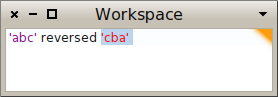
\includegraphics[width={.6}\textwidth]{workspace}
\end{center}
\subsection{The Pharo Code Browser}

\begin{center}
  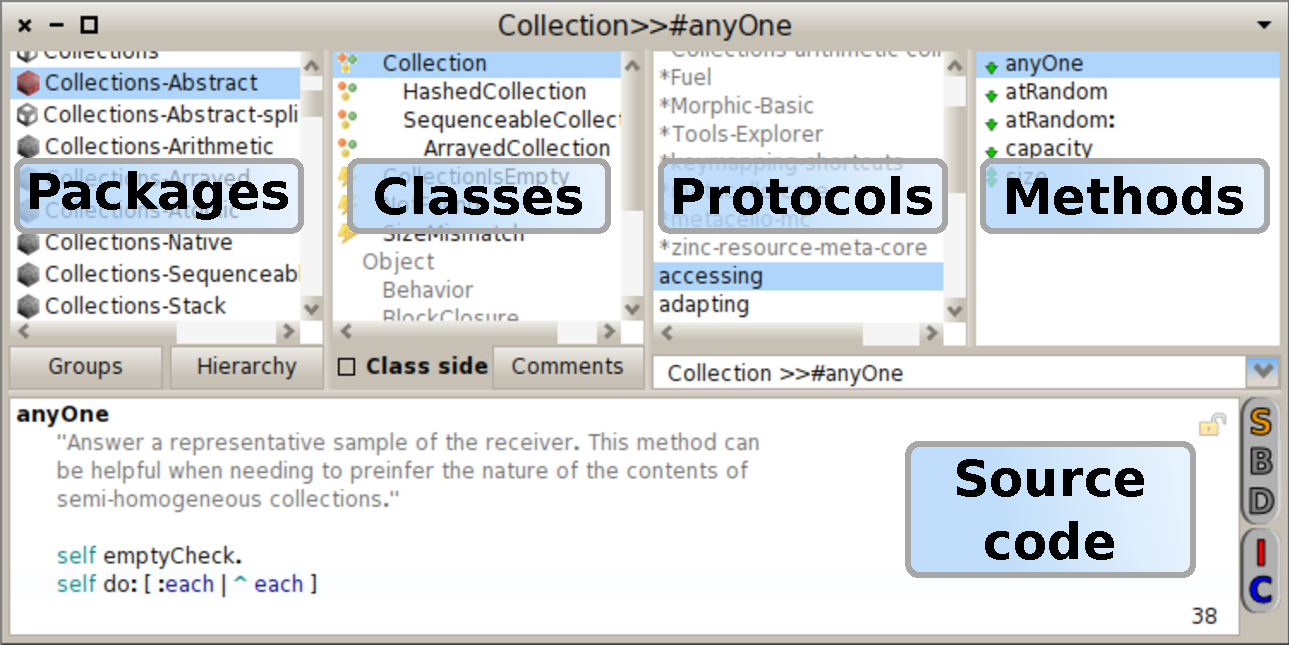
\includegraphics[width={1}\textwidth]{nautilus-anotated}
\end{center}

The Pharo code browser is composed of 5 panes:

\begin{itemize}
\item The \emph{packages} pane shows all the packages of the system or
  just a subset (by \emph{scoping} the browser);
\item The \emph{classes} pane shows a hierarchy of the classes in the
  selected package; in gray, the classes that are extended in the
  selected package but that belong to another one; the \emph{class
    side} checkbox allows for getting the methods of the meta-class of
  the selected class; the \emph{comments} button toggles the display
  of the current class's comment;
\item The \emph{protocols} pane groups the methods in the selected
  class; protocols facilitates searching for a method when the
  developer does not know its name; a protocol whose name starts with a
  \emph{*} (star) groups methods that belong to a different package
  than the one of the selected class (\eg the
  \emph{*zinc-resource-meta-core} protocol groups methods that belong
  to the \emph{zinc-resource-meta-core} package);
\item The \emph{methods} pane lists the methods of the selected
  protocol (or of the class if no protocol is selected); a down-arrow
  icon in front of a method indicates a method overridden in at least
  one subclass; an up-arrow icon indicates that the current method
  overrides one from the superclass; icons are clickable and trigger
  dedicated actions based on their meanings;
\item The \emph{source code} pane shows the source code of the select
  method; the first 3 icons on the right allows for seeing the source
  code (\emph{S}), bytecode (\emph{B}), and decompiled code
  (\emph{D}); the following 2 icons allows for browsing uses of
  instance and class variables (\emph{I} and \emph{C}).
\end{itemize}

\section{Want More?}

\subsection{Books}

The following are Pharo-specific free open-source online books:

\begin{description}
\item[Pharo By Example] http://pharobyexample.org/ (also available
  through amazon.com)
\end{description}

\end{document}

%%% Local Variables:
%%% mode: latex
%%% TeX-master: t
%%% End:
